\documentclass[12pt,a4paper]{article}
\usepackage[latin1]{inputenc}
\usepackage{float}
\usepackage{amsmath}
\usepackage{amsfonts}
\usepackage{amssymb}
\usepackage{graphicx}
\author{Luca Conterio - 920261\\
	Ibrahim El Shemy - 920174}
\date{A.Y. 2018/2019 - Prof. Di Nitto Elisabetta}



\title{%
	\textbf{\Huge{TrackMe}} \\
	\large Design Document
}

\begin{document}
	\begin{figure}
		\centering
		
\includegraphics[width=1.0\linewidth]{images/polimi}
	\end{figure}
	\maketitle

	\newpage
	\tableofcontents
	\newpage

	\section{Introduction}
	\subsection{Purpose}
	This document represents the \texttt{Design Document} (DD) for TrackMe software and contains a functional description of the system. We provide an overall guidance to the architecture of the system and it is therefore addressed to the software development team.
	\subsection{Scope}
	\texttt{TrackMe} is a company that wants to develop a software-based service allowing third parties to monitor the location and health status of individuals. Hence, the system has to be composed by two specific services:
	\begin{itemize}
	 	\item \textbf{Data4Help}\\\\
	 	This service supports the registration of individuals who agree that TrackMe acquires their data (through electronic devices such as smartwatches).
	 	\item \textbf{AutomatedSOS}\\\\ 
	 	This service is oriented to elderly people: monitoring their health status parameters, the system can send to the location of the customer an ambulance when some parameters are below certain thresholds, guaranteeing a reaction time of less than 5 seconds from the time the parameters get lower than the threshold.
	\end{itemize}
 	\subsection{Definitions, Acronyms and Abbreviations}
 		\subsubsection{Definitions}
 			\begin{itemize}
 				\item \texttt{User Device}: any compatible device with the TrackMe application, either smartphone or smartwatch.
 				\item \texttt{Personal Information}: the collection of infromation provided by a User during the registration process. It Incudes legal information, such as Social Security Number, name, surname, birth date, address, e-mail address, mobile number. Sometimes in the document this expression is abbreviated by \texttt{Data}, that also refers to clinical data.
 				\item \texttt{Assistance Request}: it is a request formulated by the system and sent to the Ambulance Dispatching System in order to guarantee users the necessary assistance.
 				\item \texttt{Individual Access Request}: sometimes referred only as \texttt{individual request} or \texttt{access request}. It refers to a singular request sent by a Third Party to a User whenever it wants to have access to User's data. It needs the User's approval. 
 				\item \texttt{Sampling Search}: it refers to a search conducted by a Third Party according to some filters, returning anonymized results for a group of people. In this document it is often called only \texttt{sampling}.
 			\end{itemize}
 		\subsubsection{Acronyms}
 			\begin{itemize}
 				\item \textbf{DD}: Design Document
 				\item \textbf{RASD}: Requirments Analysis and Specification
 				\item \textbf{ERP}: Enterprise Resource Planning
 				\item \textbf{DMZ}: Demilitarized Zone
 				\item \textbf{RAPS}: Reliable Array of Partitioned Service
 				\item \textbf{API}: Application Programming Interface
 				\item \textbf{DBMS}: Database Management System
 			\end{itemize}
 		\subsubsection{Abbreviations}
 		
 	\newpage
	\subsection{Document Structure}
		\begin{itemize}
			\item \textbf{1 Introduction}\\\\
			This section introduces the Design Document. It explains the Purpose, the Scope and the framework of the document.
			\item \textbf{2 Architectural Design}\\\\
			This section is focused on the main components used for this system and the relationship between them, providing information about their deployment and how they operate. It also focuses on the architectural styles and the design patterns adopted for designing the system.
			\item \textbf{3 User Interface Design}\\\\
			This section provides an overview on how the User Interface will look like and furthermore gives a more detailed extension using UX and BCE diagrams.
			\item \textbf{4 Requirments Traceability}\\\\
			This section explains how the requirements defined in the RASD map to the design elements defined in this document.
			\item \textbf{5 Implementation, Integration and Test Plan}
		\end{itemize}
\newpage
\section{Architectural Design}
	\subsection{High Level Components and their Interactions}
	\begin{figure}[h]
		\centering
		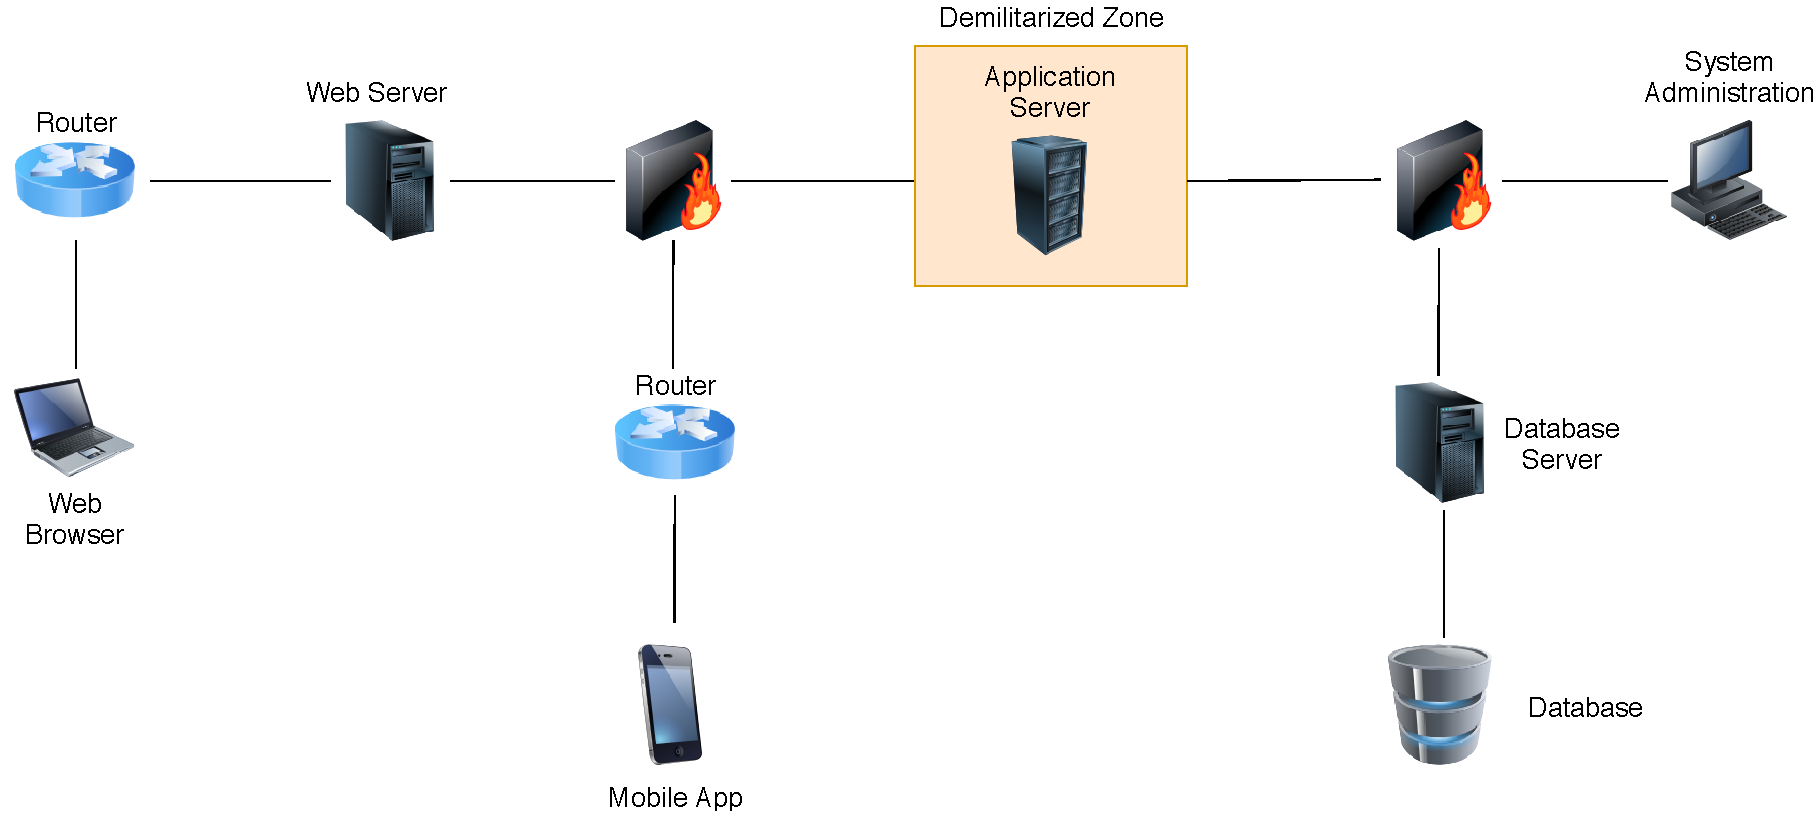
\includegraphics[height=0.5\linewidth]{images/high_level_diag}
		\caption{High Level System Structure}
		\label{fig:highleveldiag} 
	\end{figure}


The architecture of our system can be streamlined into 3 logic layers:
	\begin{itemize}
		\item \textbf{Presentation Layer}\\ 
		This layer can be divided into the Client tier (that includes the Web App and the Mobile App) and the Web tier. Third parties can access the system's functionalities and Users' information to which they are subscribed to through the Web Server. 
		\item \textbf{Application Layer}\\
		Users logged into the Mobile Application can access the system's functionalities and communicate with the Application Server, located in a Demilitarized Zone (DMZ), directly.
		\item \textbf{Data Layer}\\
		On top of that, we have the Database Server and the Database itself, where data about registered Users and Third Parties are stored and managed.
	\end{itemize}
	System Administration is implemented through a third-party ERP solution, hence we do not provide information about its implementation.
	
	\subsection{Component View}
		\subsubsection{High Level Component Diagram}	
			The following diagrams illustrate the system components and the interfaces through which they interact to fullfil their functionalities. A distinction can be made between Client side and Server side:
			\begin{itemize}
				\item The Client side is composed by two components, \texttt{Web Application} and \texttt{Mobile Application},  referring to the following services:\\
				\texttt{ThirdPartiesWebServices} and \texttt{UserMobileServices}.
				
				\item The Server side is composed of two main components, \texttt{Third Parties web services} that will provide functionalities aiming to fullfill third parties needs, such as sending requests to Users, \texttt{User mobile services} that will provide an interface to User in order to manage his own profile, check information about his health status, accept/reject requests, etc.
			\end{itemize}
			
			\begin{figure}[h]
				\centering
				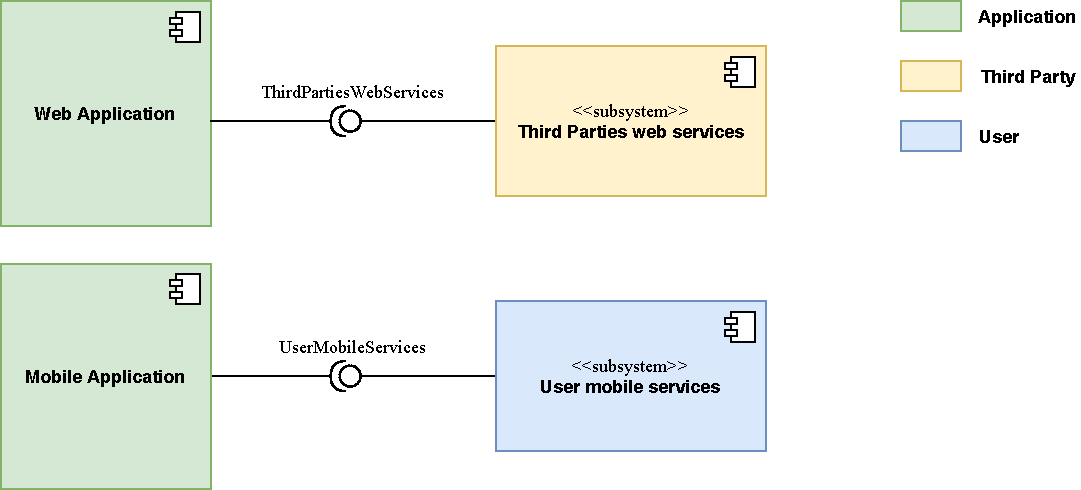
\includegraphics[width=1.0\linewidth]{images/high_lvl_comp_diag}
				\label{fig:highlvlcompdiag}
			\end{figure}
	
		\newpage
		\subsubsection{User Mobile Services Projection}
			User Mobile Services subsystem is composed by five components: \texttt{Activity Tracker Module}, \texttt{Health Monitoring Module}, \texttt{SOS Assistance Module}, \texttt{Access Requests Module} and \texttt{Profile Manager Module}. These components provide to the User Mobile Application the following interfaces: \texttt{ActivityTracker}, \texttt{HealthMonitor}, \texttt{AssistanceRequestHandler}, \texttt{RequestHandler} and \texttt{ProfileManager}. The components need also to communicate with \texttt{Google Maps}, \texttt{Google Sensors}, \texttt{Google Notifications}, \texttt{Ambulance Dispatching System}, \texttt{SMS gateway} and the \texttt{DBMS} to work properly and guarantee a better User experience with the Application.
			\begin{figure}[H]
				\centering
				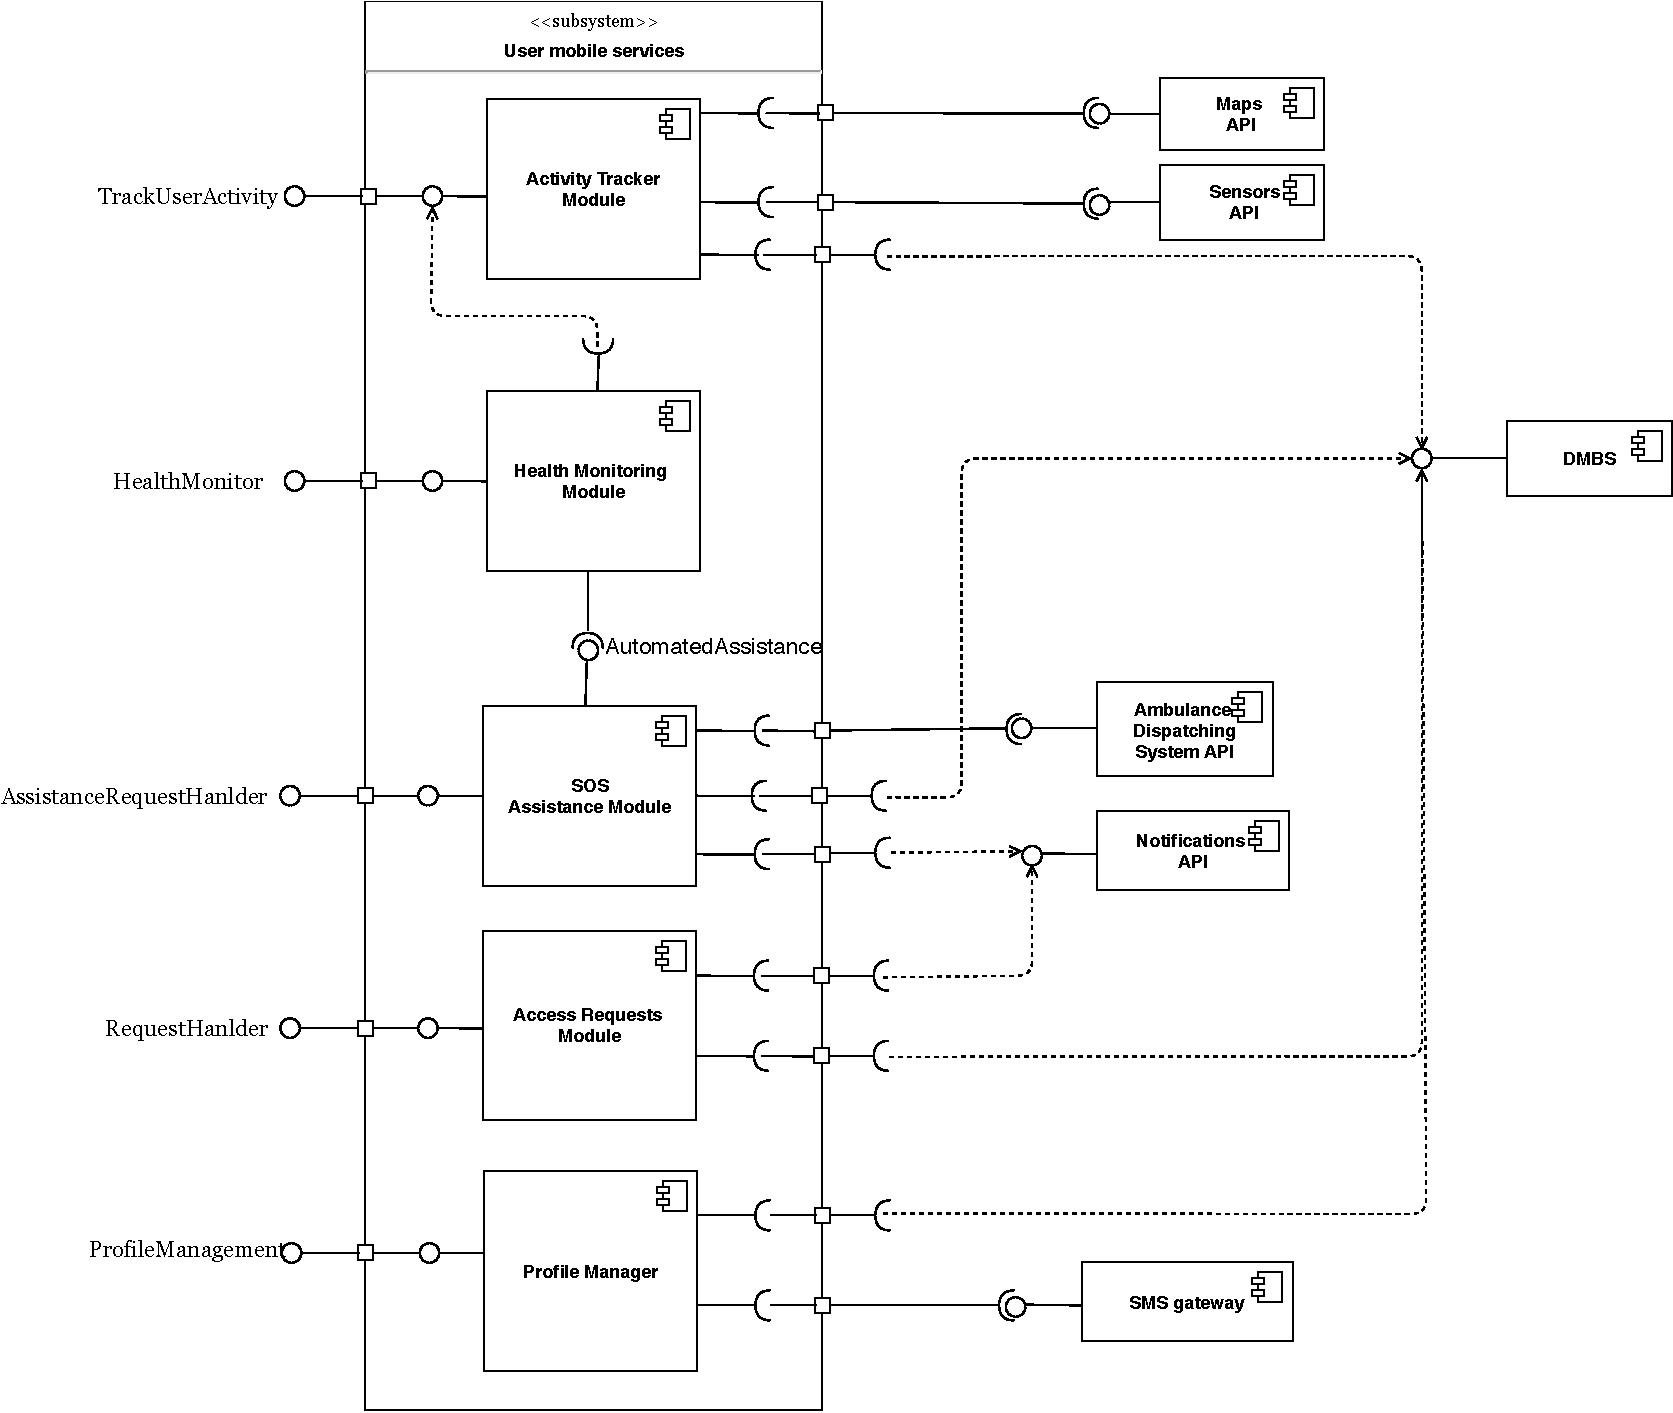
\includegraphics[height=1.0\linewidth]{images/user_projection}
				\label{fig:user_projection}
			\end{figure}
			\newpage
			For what concerns smartwatches, the server will not distinguish between messages and requests received directly by the smartwatch device (e.g. if it is equipped with GPS) and those retrieved by the sensors and forwarded to the server thanks to the connectivity of a smartphone.
			The User Mobile Services subsystem will handle all the mentioned situations.\\
			The only difference is that the smartwatch interface will not provide the user the possibility to manage his/her profile, since it would not be user friendly nor comfortable.
		
			\subsubsection*{Module Functionalities}
				\begin{itemize}
					\item \texttt{Activity Tracker Module}: this module is devoted to everything that concerns data retrieved by user's devices, such as location, steps, covered distance, heartbeat, blood pressure and sleep.
					\item \texttt{Health Monitoring Module}: this component persists in an idle state as long as a user is not registered to AutomatedSOS service.\\
					Otherwise, it interpellates directly the Activity Tracker Module, through the ActivityTracker interface in order to check the user's health status. Moreover, thanks to the AutomatedAssistance interface it can ask for an automated assistance request.
					\item \texttt{SOS Assistance Module}: in this module all functions dealing with assistance requests are implemented. It directy handles on-demand assistance requests and automated assistance requests performed by the Health Monitoring Module through the AutomatedAssistance interface.
					\item \texttt{Access Requests Module}: this component handles the access requests coming from some third parties, that want to have access to the user's data, giving the user the possibility to accept or reject them. It also manages the updates performed by the user to the permissions given to the third parties.
					\item \texttt{Profile Manager Module}: it provides all the functions concerning the user authentication and the update of profile informations.
				\end{itemize}
		
		\newpage
		\subsubsection{Third Party Web Services Projection}
				 Third Party Web Services subsystem is composed by five components: \texttt{Data Access Module}, \texttt{Subscription Module}, \texttt{Access Requests Module}, \texttt{Sampling Requests Module} and \texttt{Authentication Manager Module}. These components provide to the Web Application the following interfaces: \texttt{DataAccessManager}, \texttt{SubscriptionManager}, \texttt{RequestProvider} and \texttt{AuthenticationManager}. The components need also to communicate with \texttt{Google Notifications} and the \texttt{DBMS} to work properly.
			\begin{figure}[H]
				\centering
				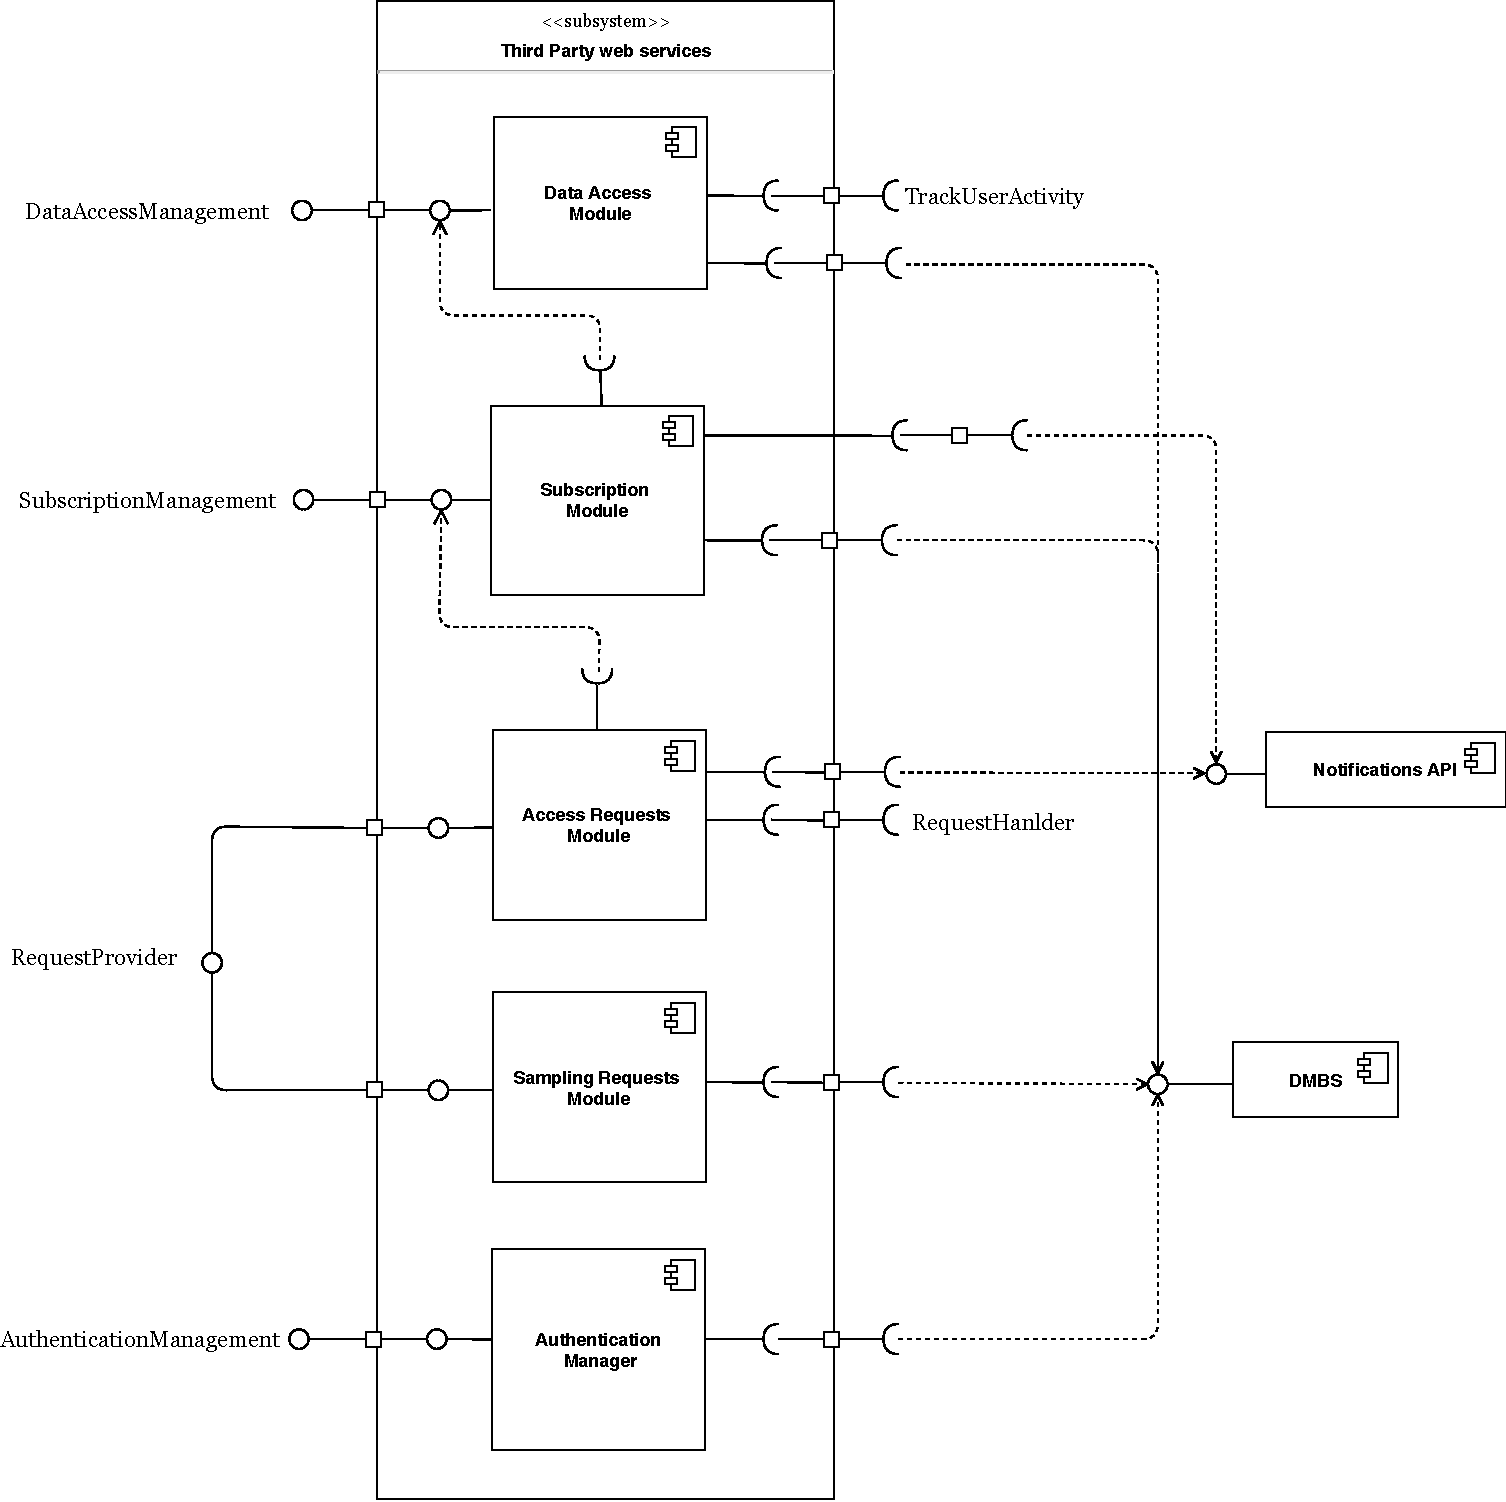
\includegraphics[height=1.0\linewidth]{images/third_party_projection}
				\label{fig:third_party_projection}
			\end{figure}
			\newpage
			\subsubsection*{Module Functionalities}
				\begin{itemize}
					\item \texttt{Data Access Module}: it deals with accessing to user's data, in case of the specific third party has access to him/her.
					\item \texttt{Subscription Module}: this component is responsible for subscribing a third party to a specific user, after the access request has been accepted. If the operation terminates successfully it checks the existence of new data retrieved by the Data Access Module and notifies the involved third party, thanks to the Notifications API.
					\item \texttt{Access Requests Module}: it provides the third party with an interface that allows it to send data access request to a specific user.
					If a request is accepted, it also gives the possibility to the third party to subscribe to user's new data.
					\item \texttt{Sampling Requests Module}: similar to the Access Requests Module, provides an interface to allow the third party retrieving anonymized information of a group of users.
					\item \texttt{Authentication Manager Module}: this module provides all functionalities concerning with the registration and login of a third party to the system.
				\end{itemize}
		
		\newpage
		\subsection{Deployment View}
				For the deployment of the system, we opted for a 4-tier architecture composed as follows:
				\begin{itemize}
					\item \textbf{Tier 1}\\
					This tier is composed by the Client (implemented as a Thin Client), that includes the Web App (run by a web browser) and the Mobile Application (run by smartphones). 
					\item \textbf{Tier 2}\\
					This tier is composed by the Web Server, whose main functionality is to store, process static content and deliver web pages to the Clients. For this reason, we opted for NGINX, that guarantees better perfomances for static content processing. It can be also configured as a load balancer, in order to better handle multiple connections.
					\item \textbf{Tier 3}\\
					This tier corresponds to the Application Server, that provides both facilities to create web applications and a server environment to run them. We opted for WildFly (v. 12.0.0 or recent versions - previously JBoss) since it fully implements all Java EE specifications.
					\item \textbf{Tier 4}\\
					This tier corresponds to the Database Server on which the DBMS is running. We opted for MySQL (v. 8.0.12) since it is one of the most secure and reliable database management system used in popular web applications and guarantees scalability and high performance.
				\end{itemize}
	
			As mentioned briefly in the RASD (sections 3.9.2, 3.9.5), our system has to rely on a RAPS architecture, in order to prevent unavailability of some functionalities in case of breakdowns. This architecture consists in a partitioned and redundant structure: servers are cloned to achieve this objective.
			More precisly, multiple services are divided on different machines and each machine can access in turn to a copy of the stored data. Such architecture guarantees better availability and scalability and provides a high rate of maintainability: in case of breakdowns, it is sufficient to work on the damaged machine, without interfering with the other machines' tasks, while the specific service can still be perfomed. 
			In addition, if the system is willing to expand some services, it is sufficient invest on the specific partition associated to that service.
			\begin{figure}[H]
				\centering
				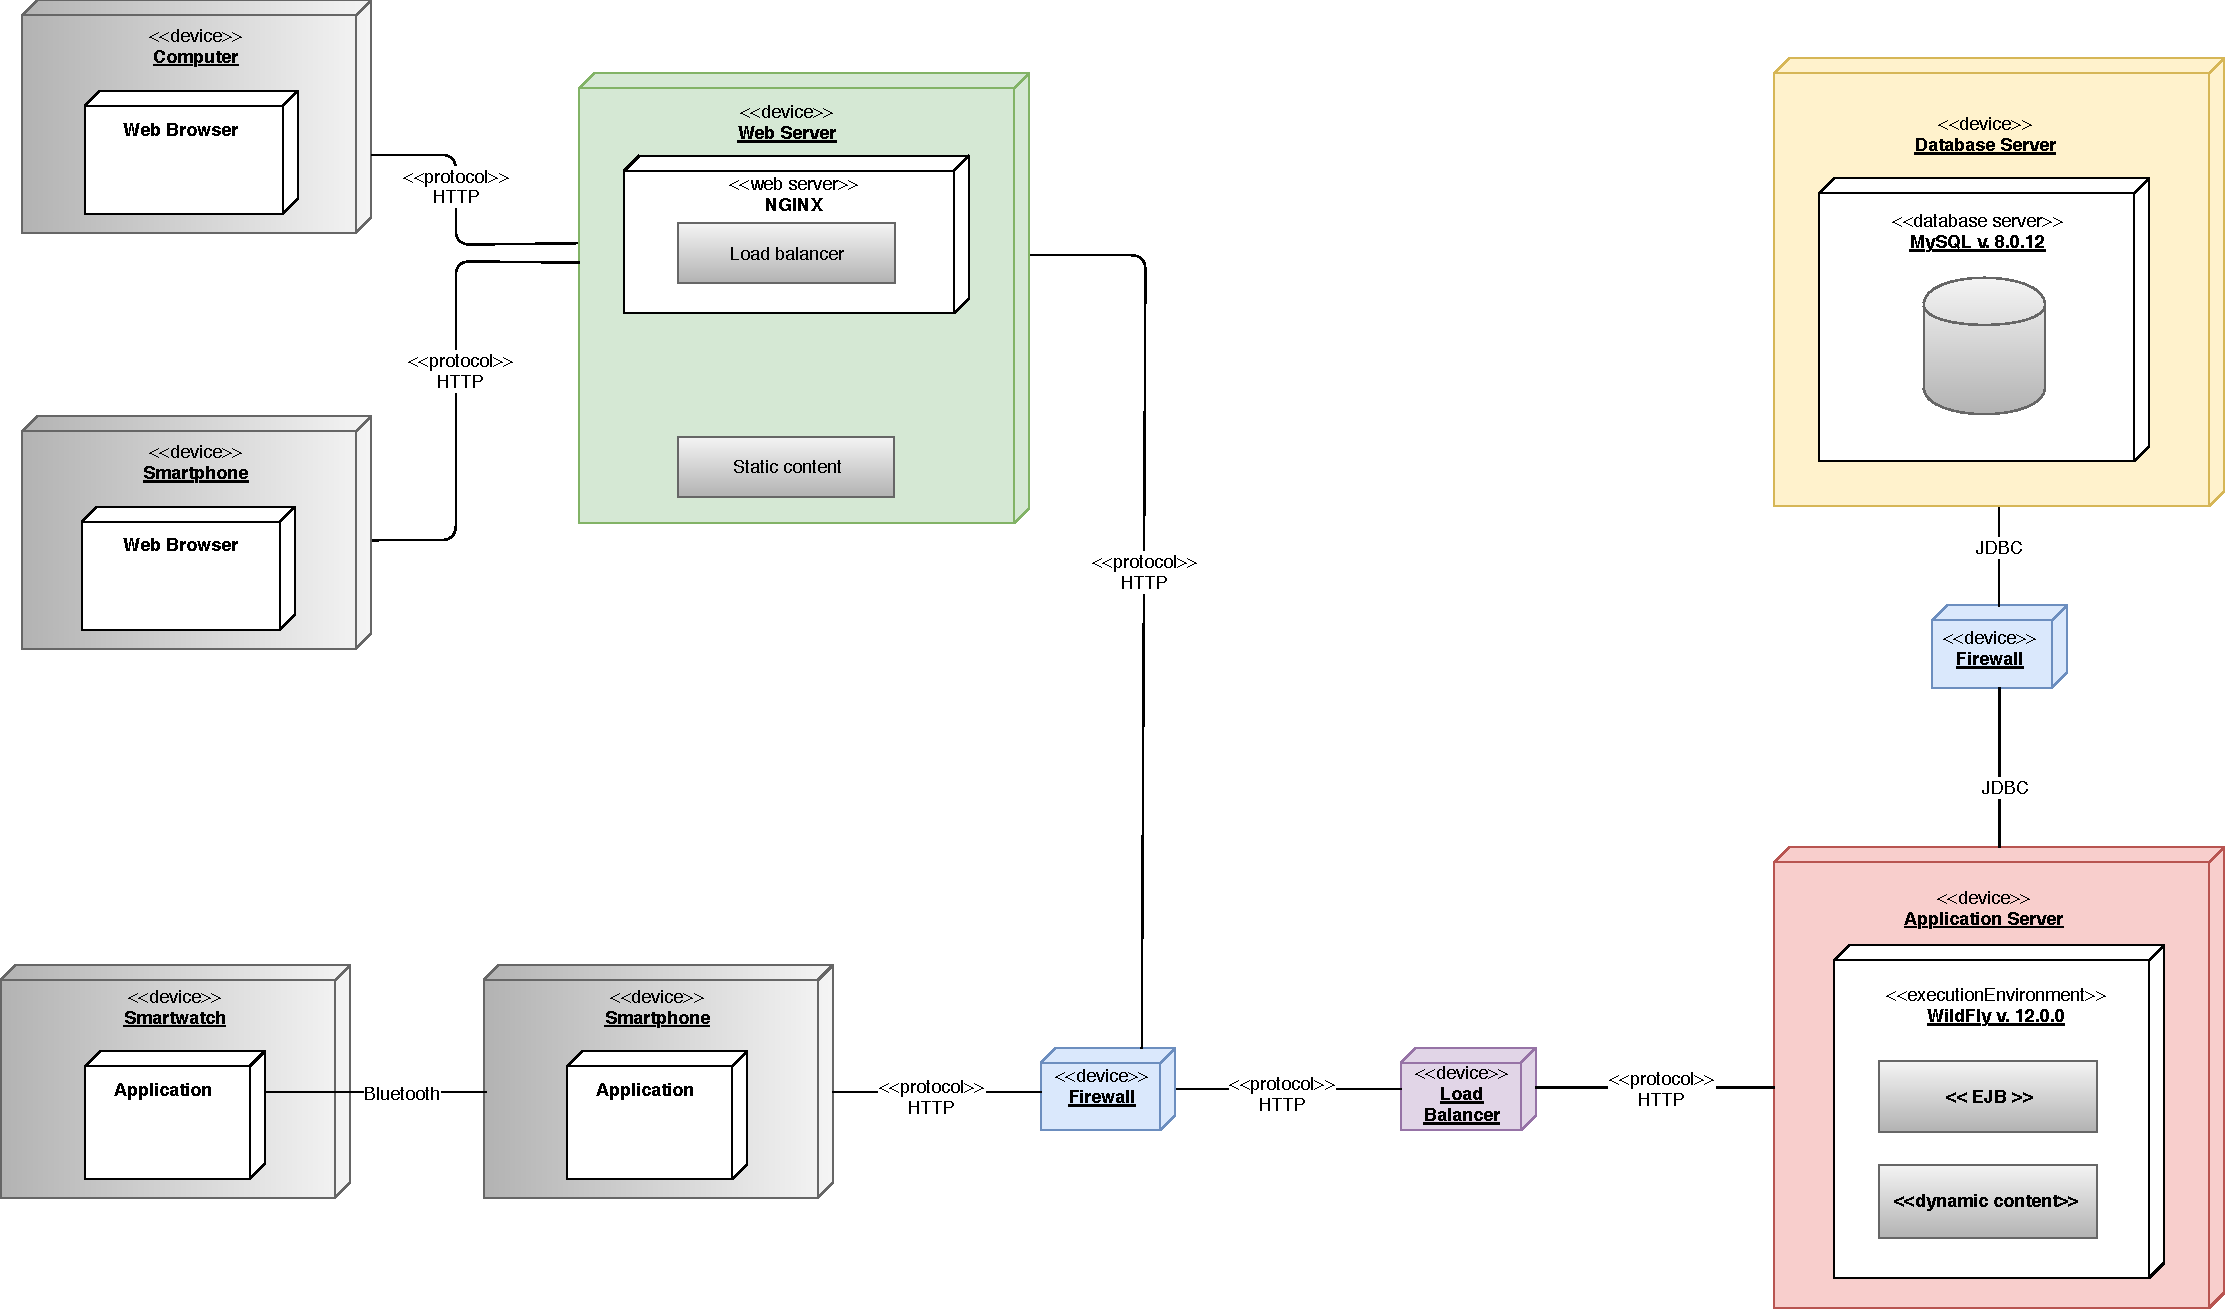
\includegraphics[width=1.0\linewidth]{images/deployment_diagram}
				\caption{Deployment View Diagram}
				\label{fig:deployment_diagram}
			\end{figure}
			\begin{figure}[H]
				\centering
				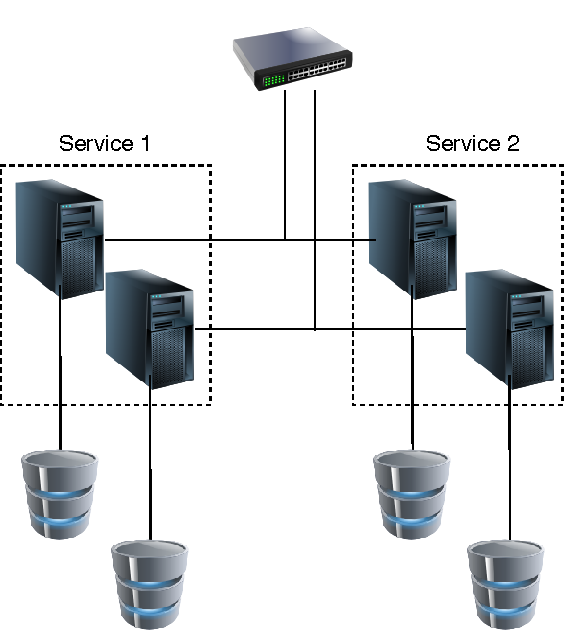
\includegraphics[width=0.6\linewidth]{images/raps}
				\caption{RAPS Architecture}
				\label{fig:raps}
			\end{figure}
		
		\newpage
		\subsection{Component Interfaces}
			\begin{figure}[H]
				\centering
				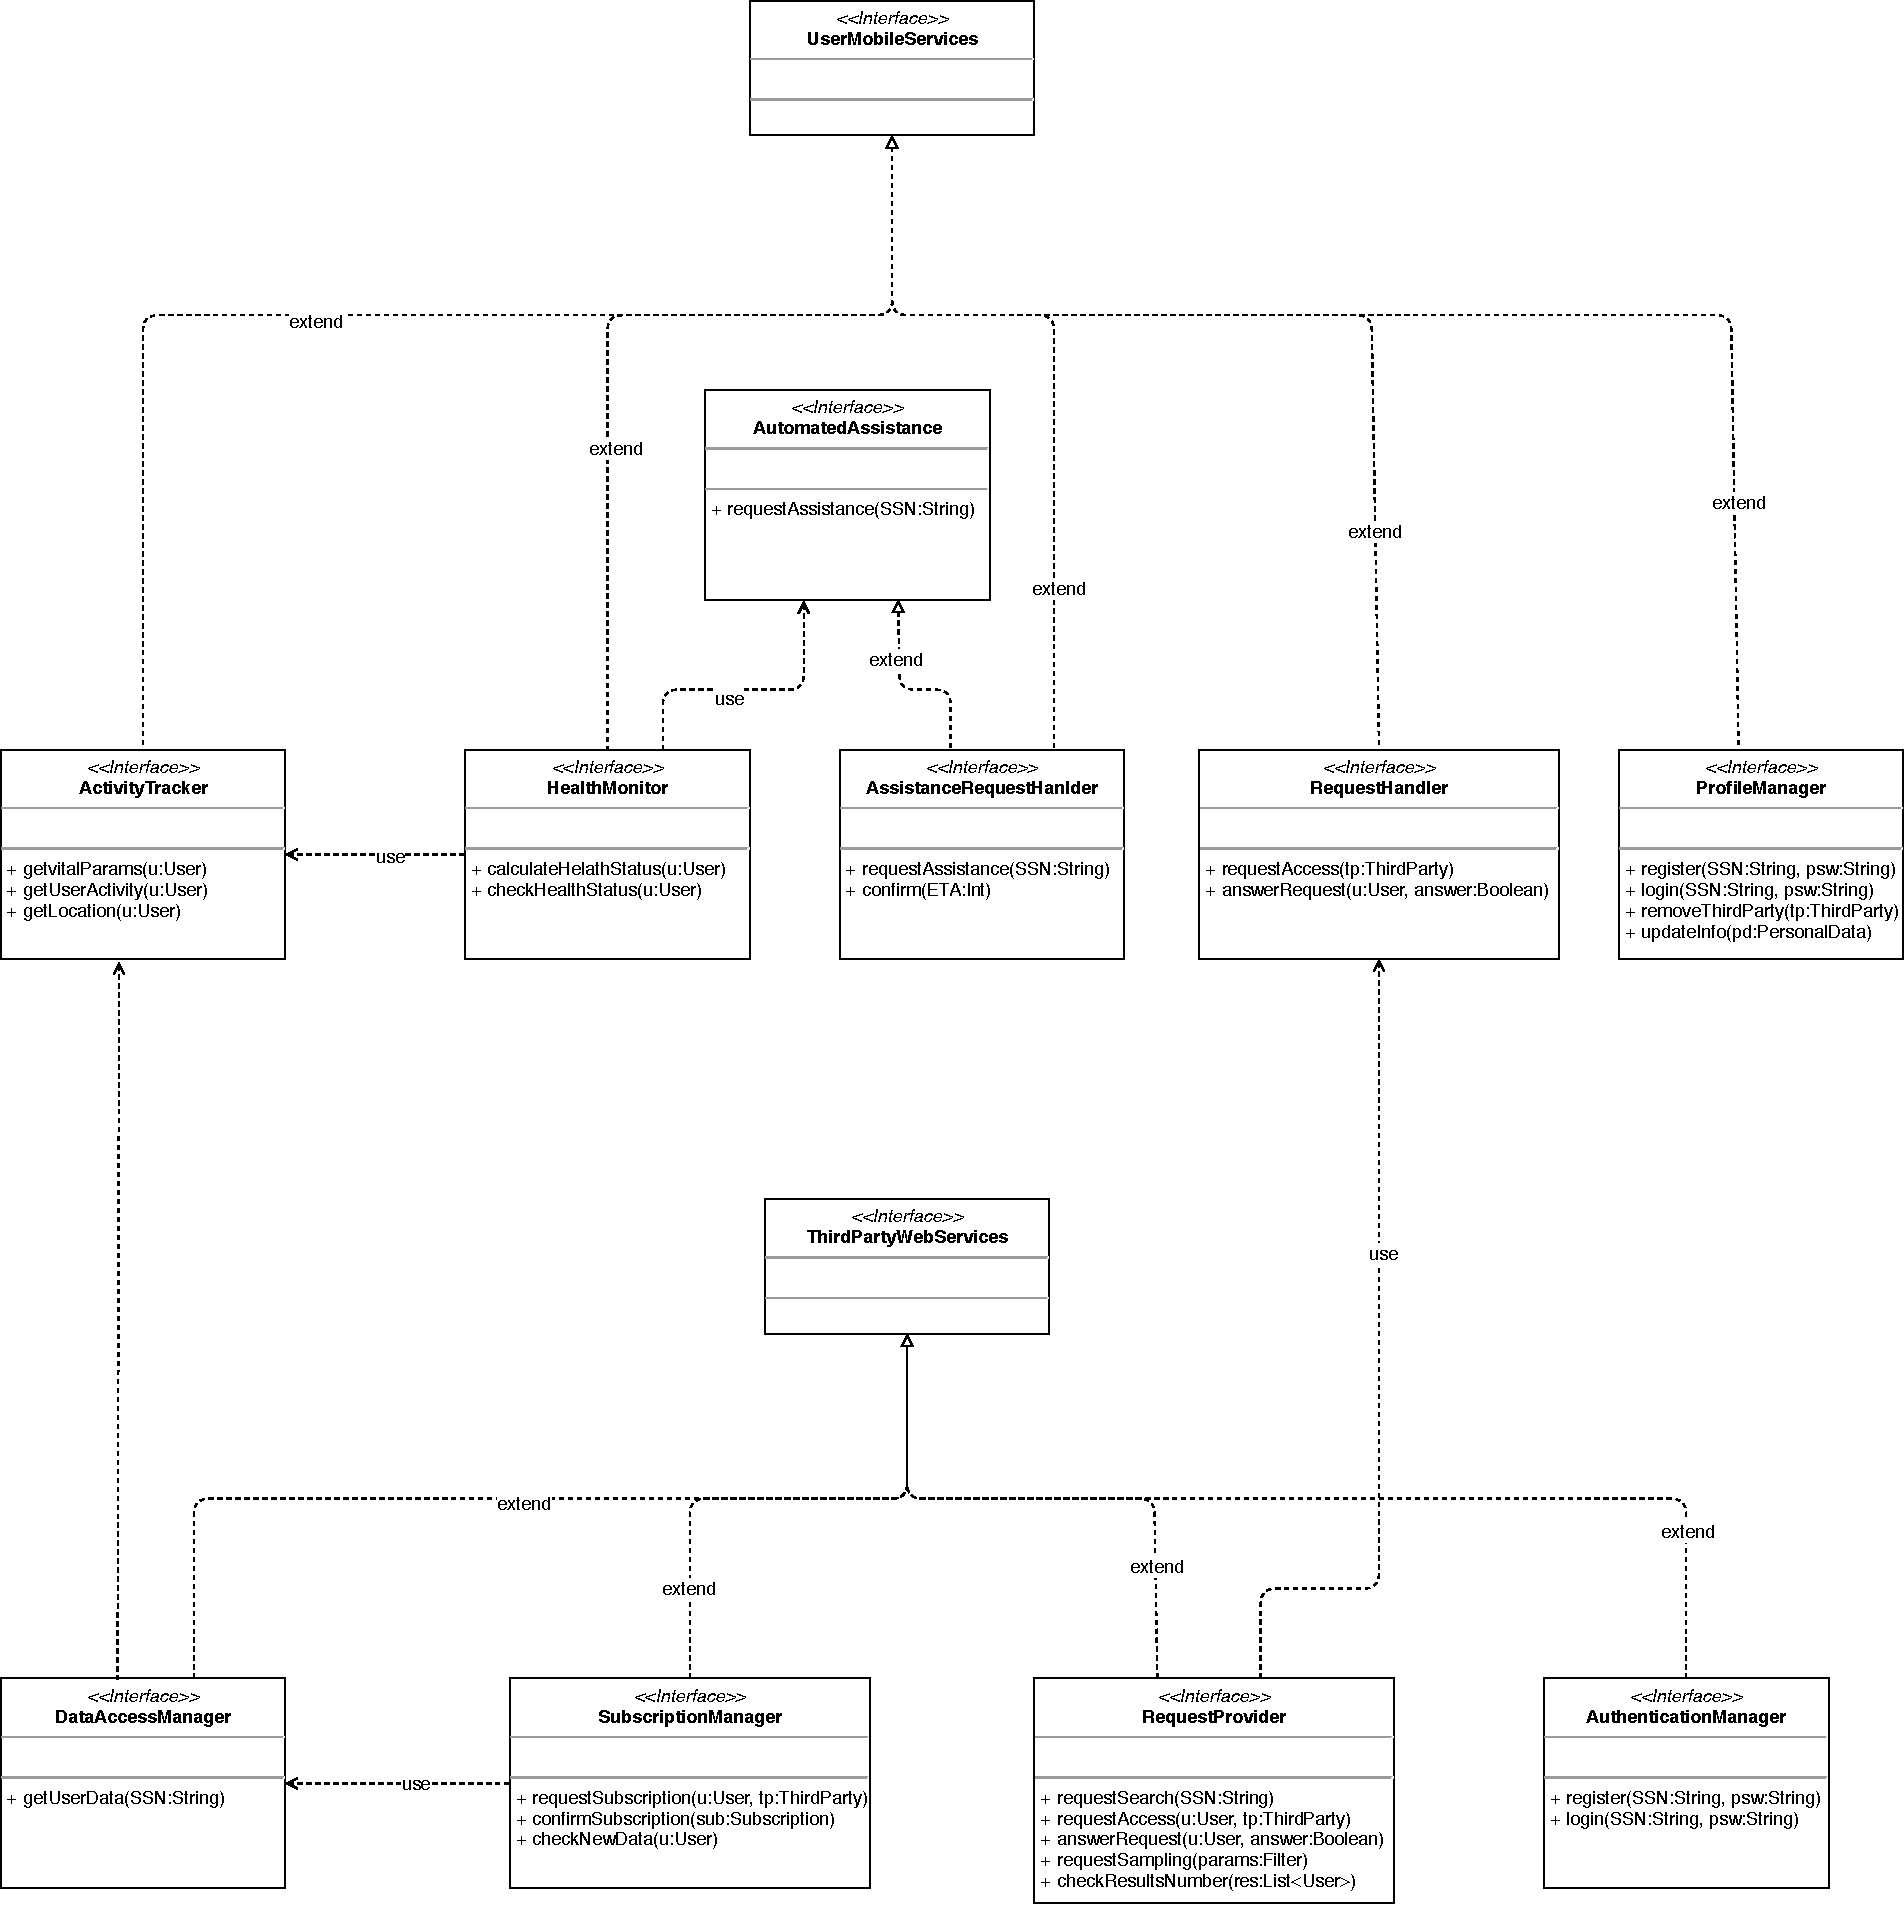
\includegraphics[height=1.2\linewidth]{images/comp_interfaces}
				\caption{Component interfaces and their interactions.}
				\label{fig:comp_interfaces}
			\end{figure}
		
		\newpage
		\subsection{Runtime View}
		
		\newpage
		\subsection{Architectural Styles and Design Patterns}
			\subsubsection{Design Patterns}
			In order to better formalize our architecture and make it as flexible as possible and speed up the devolpment process of our system we used different design patterns:
			\begin{itemize}
				\item \textbf{Model View Controller}\\ 
				The majority of Mobile and Web applications rely on this pattern. In fact, these applications retrieve data from a data collector (generally a Database) and update the User Interface, according to the input provided and the validity of the requested operation is checked by the Controller.\\
				Thus, the main key of this pattern is to create a separation between the User Interface (View), the data (Model) and the response and validity checking of the User's input (Controller).
				\item \textbf{Observer and Observable}\\
				In this pattern, there are many observers (objects) which are observing a particular subject (observable object). Observers are basically interested and want to be notified when there is a change made inside that subject. So, they register themselves to that subject. When they lose interest in the subject they simply unregister from the subject. In our system, the intent of this pattern is to let the User execute some query through the UI and after searching the Database, the result is reflected back in the UI. In most of the cases we segregate the UI with the Database. If a change occurs in the database, the UI should be notified so that it can update its display according to the change. When a change is occurring an event is notified and the changes are applied and updated for the User.
				\item \textbf{Visitor Pattern}\\
				This pattern's main purpose is to abstract functionalities that can be applied to an aggregate hierarchy of 'element' objects. In particular, we adopted this pattern in order to handle events that notify changes to the User Interface (View component). This way, we create a double dispatching mechanism, and the Controller is able to recognize the event type and associate correctly the requested operation.
				\item \textbf{Fa�ade Pattern}\\
				This design pattern supports loose coupling. In fact we emphasize the abstraction and hide complex details by exposing a single interface instead of multiple ones. According to our system we expose to the client \texttt{ThirdPartyWebServices}, \texttt{UserMobileServices} and \texttt{UserSmartwatchServices} that are in turn extended respectively by all the interfaces provided by the subsystems Third Party Web Services, User Mobile Services and User Smartwatch Services (see section 3, Component View).
				\item \textbf{Proxy Pattern}\\
				It provides a surrogate for another object to control access to it. In our system architecture it can be useful to interface the Application Server with the Database Server. For example, whenever a user or a third party requests some data that is unchanged, the proxy can answer the query without involving access to the database, providing a better response time. 
			\end{itemize}
		
		\newpage
		\subsection{Other Design Decisions}
		
	\newpage
	\section{User Interface Design}
	
	\newpage
	\section{Requirements Traceability}
	
	\newpage
	\section{Implementation, Integration and Test Plan}
		
	\newpage
	%\section{Appendix}
	\section{Effort Spent}
	\begin{itemize}
		\item Luca Conterio
		\begin{center}
			\begin{tabular}{| c | c | c |}
				\hline
				Day & Subject & Hours \\ \hline
				19/11/2018 & High Level Components & 1.5 \\ \hline
				22/11/2018 & Component View & 1.5 \\ \hline
				25/11/2018 & Component View & 3 \\ \hline
				26/11/2018 & Deployment View & 2.5 \\ \hline
				Total &									& \\ \hline
			\end{tabular}
		\end{center}

		\item Ibrahim El Shemy
		\begin{center}
			\begin{tabular}{| c | c | c |}
				\hline
				Day & Subject & Hours \\ \hline
				19/11/2018 & Introduction of the document & 1.5 \\ \hline
				22/11/2018 & Component View & 2.5 \\ \hline
				25/11/2018 & Component View & 3 \\ \hline
				26/11/2018 & Deployment View and Design Patterns & 2.5 \\ \hline
				Total &									& \\ \hline
			\end{tabular}
		\end{center}
	\end{itemize}
	\section{References and Used Tools}
		\subsection{Reference Documents}
			\begin{itemize}
				\item Specification Document "Mandatory Project Assignment A.Y. 2018/2019"
				\item "Appunti di Sistemi Informativi per il Settore dell?Informazione" A.Y. 2017/2018
				\item "Java Design Patterns", Vaskaran Sarcar
			\end{itemize}
		\subsection{Tools}
			\begin{itemize}
				\item \textbf{Draw.io}: \texttt{https://www.draw.io/}
				\item \textbf{TeXStudio}: \texttt{http://www.textstudio.org/}
				\item \textbf{Github}: \texttt{https://github.com/}
			\end{itemize}
		
\end{document}
